\documentclass[12pts]{report}

\usepackage[margin=1in]{geometry}
\usepackage[usenames, dvipsnames]{color}
\usepackage{setspace}
\usepackage{graphicx}
\doublespacing
\usepackage{fancyvrb}
\usepackage{varwidth}
\usepackage{verbatim}
\usepackage{multicol}
\usepackage{hyperref}

\usepackage{parskip}                    % This packages sets the spacing between two paragraphs
\setlength{\parskip}{.5\baselineskip}   % Define spacing between two paragraphs

\setlength{\parindent}{0pt}
\setlength{\columnseprule}{1pt}

% Title Page
\title{DIME DYNAMIC DOCUMENTATION TRAINING }
\author{Luiza Andrade \& Mrijan Rimal} 
\date{\today}


\makeatother


\begin{document}
	

\makeatletter
\begin{titlepage}
	\begin{center}
		
\includegraphics[width=0.3\linewidth]{i2i.png}\\[10ex]
		{\LARGE \bfseries  \@title }\\[2ex] 
		{\Large  \@author}\\[20ex] 
		{\large \@date}
	\end{center}
\end{titlepage}
\makeatother

\section*{Introduction}
{\LaTeX} is a very useful tool to display descriptive statistics and analysis results. It allows us to create a document once and every time a do-file is run, the tables are automatically updated in our LaTeX document. 

To complete these tasks, you should use the \textcolor{red}{Add path and name of do-file} do-file and \textcolor{red}{Add path and name of template} {\LaTeX} template provided on the DIME dynamic documentation folder. There's no need to download any datasets. If you prefer, you can also use your own dataset, but in that case the do-file should also be adapted. 

The templates in the folder should allow you to do all you are asked in these exercises, but if you want to have a more broad understanding of {\LaTeX} or explore other functionalities, this \href{https://en.wikibooks.org/wiki/LaTeX
}{{\LaTeX} Wikibook} is a great source. For more specific questions about how to perform a task or solve an error, Google usually has the answer.

\textbf{Exercise Objectives:} Learn how to present tables and graphs in a {\LaTeX} document.

\section*{Exercise 1. Set up folders}

\section*{Exercise 2. Exporting Tables}
Open \textcolor{red}{Export tables and images.do} and change the paths on the first section of the do-file so that it matches the folder structure you just created. Then run the do-file. This will export a few tables and graphs to the Raw folder that will be used in the following exercises. If you want to take a step back and review how to export tables and images from Stata, the a look at the folder called "Excercise Stata - How to export tables and graph from Stata to LaTeX".

\section*{Exercise 3. Using TeXstudio interface to import an image into \LaTeX}
Open Exercise 1.tex. This is a very basic {\LaTeX} document and consists on the initial settings we will build on. You will add lines between \verb|\begin{document}| and \verb|end{document}| to create your document content.


The first thing we want to do is to figure out the path to the files we want to import. {\LaTeX} uses relative paths, which means they must start in the very same folder as the .tex file you are editing is, which can be a little tricky if you're not used to it. So we'll use a shortcut to find out what it is.

Open the Raw folder where your tables and figures were saved, then click iegraph.png and drag it to Exercise 1.tex, placing it just below the line that says "This is a blank document". Then click "OK". This will create something similar to

\begin{center}
\begin{Verbatim}[commandchars=+\(\)]
	\begin{figure}
		\centering
		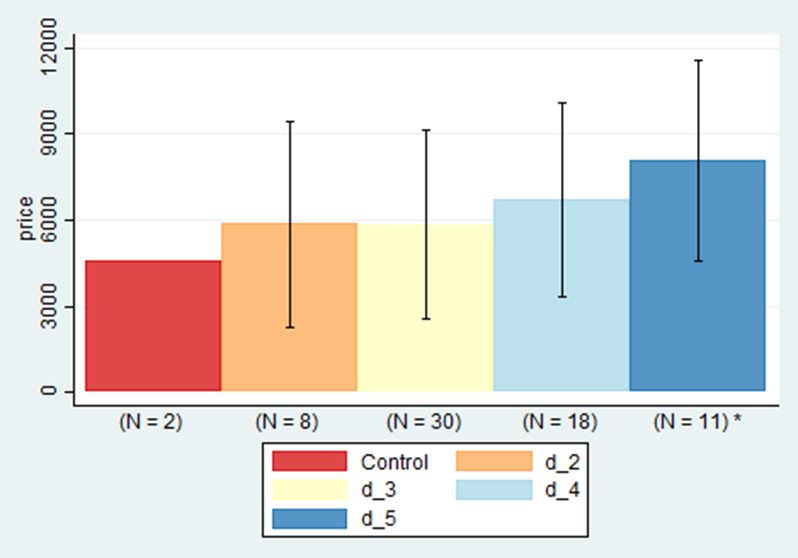
\includegraphics[width=0.7\linewidth]{Raw/iegraph}
		\caption{}
		\label{fig:i2i}
	\end{figure}
\end{Verbatim}
\end{center}

The path to your "Raw" folder is what appears inside the curly braces after \verb|\includegraphics|. In this example, it is just \color{red}{\verb|Raw/|}\color{black}{.}

\section*{Exercise 4. Manually importing graphs into \LaTeX}

Now we want to manually import a figure to that same .tex file, just so we can understand what is being done by the lines of code that TeXstudio created.

\textbf{Task 1:} Create a figure environment and import regular\_graph.png into it. This can be done by typing the following lines below your iegraph:

\begin{center}
	\begin{Verbatim}[commandchars=+\(\)]
	\begin{figure}[H]
		\includegraphics{+color(red)Raw/+color(black)regular_graph.png}
	\end{figure}
	\end{Verbatim}
\end{center}

Remember to replace \color{red}{\verb|Raw/|}\color{black}{} by the file path to your "Raw" folder. How does it look? 

\textbf{Task 2:} Adjust the size of your figure so it fits into the page. Use the \verb|\width| option of \verb|\includegraphics{}| to do this by typing the context in blue:
\begin{center}
	\begin{Verbatim}[commandchars=+\(\)]
	\begin{figure}[H]
		\includegraphics+color(CornflowerBlue)([width=\textwidth])+color(black)({Raw/regular_graph.png})
	\end{figure}
	\end{Verbatim}
\end{center}


\textbf{Task 3:} Center your figure by adding the line in blue:
\begin{center}
	\begin{Verbatim}[commandchars=+\(\)]
	\begin{figure}[H]
	+color(CornflowerBlue)(\centering)
		\includegraphics[width=\textwidth]{Raw/regular_graph.png}
	\end{figure}
	\end{Verbatim}
\end{center}

\textbf{Task 4:} Add a title to your figure using the \verb|\caption| command:
\begin{center}
	\begin{Verbatim}[commandchars=+\(\)]
	\begin{figure}[H]
	\centering
		\includegraphics[width=\textwidth]{Raw/regular_graph.png}
		+color(CornflowerBlue)\caption{Add figure title here}
	\end{figure}
	\end{Verbatim}
\end{center}

\section*{Exercise 5. Importing Tables into \LaTeX}
\textbf{Task 1:} Create a table environment and import regression\_table.tex into it. This can be done by typing the following lines below your regular\_graph:
\begin{center}
	\begin{Verbatim}[commandchars=+\(\)]
	\begin{table}[H]
		\input{+color(red)Raw/+color(black)regression_table.tex}
	\end{table}
	\end{Verbatim}
\end{center}

\begin{center}
	\textcolor{BurntOrange}{\emph{Tip:} don't forget to substitute the path to your Raw folder.}
\end{center}
		
\textbf{Task 2:} Use \verb|\AdjustBox| to adjust table size. You can do this by adding the lines in blue: 
	\begin{center}
	\begin{Verbatim}[commandchars=+\(\)]
	\begin{table}[H]
	+color(CornflowerBlue)(\begin{adjustbox}{max width=\textwidth})  
		{
\def\sym#1{\ifmmode^{#1}\else\(^{#1}\)\fi}
\begin{tabular}{l*{8}{c}}
\hline\hline
                    &\multicolumn{1}{c}{(1)}&\multicolumn{1}{c}{(2)}&\multicolumn{1}{c}{(3)}&\multicolumn{1}{c}{(4)}&\multicolumn{1}{c}{(5)}&\multicolumn{1}{c}{(6)}&\multicolumn{1}{c}{(7)}&\multicolumn{1}{c}{(8)}\\
                    
\hline
Post        &      -0.304\sym{*}  &      -0.632\sym{***}&       0.003         &       0.217\sym{**} &      -0.059         &      -0.012         &       0.136         &       0.333         \\
                    &     (0.141)         &     (0.026)         &     (0.130)         &     (0.072)         &     (0.082)         &     (0.029)         &     (0.365)         &     (0.265)         \\
[1em]
Treatment     &      -0.055         &       0.267\sym{***}&      -0.133\sym{*}  &       0.096         &      -0.210\sym{*}  &      -0.035         &      -0.117         &      -0.033\sym{***}\\
                    &     (0.152)         &     (0.000)         &     (0.064)         &     (0.105)         &     (0.098)         &     (0.078)         &     (0.133)         &     (0.000)         \\
[1em]
Post * treatment &               &               &       0.065         &      -0.254\sym{*}  &       0.111         &      -0.000         &       0.284         &      -0.585         \\
                    &                 &                &     (0.159)         &     (0.116)         &     (0.086)         &     (0.033)         &     (0.378)         &     (0.296)         \\
[1em]
Constant            &       0.581\sym{***}&       0.333\sym{***}&       0.378\sym{***}&       0.175         &       0.276\sym{**} &       0.039         &       0.364\sym{**} &       0.000         \\
                    &     (0.131)         &     (0.000)         &     (0.055)         &     (0.105)         &     (0.095)         &     (0.081)         &     (0.115)         &     (0.000)         \\
\hline
Observations        &         354         &         354         &        1897         &        1897         &        1652         &        1652         &         348         &         348         \\
Fixed-effects  &          No         &         Yes         &          No         &         Yes         &          No         &         Yes         &          No         &         Yes         \\

\(R^{2}\)           &       0.033         &       0.595         &       0.014         &       0.287         &       0.043         &       0.386         &       0.076         &       0.535         \\

\hline\hline
\multicolumn{9}{l}{\footnotesize Standard errors clustered at user level are in parentheses. \sym{*} \(p<0.05\), \sym{**} \(p<0.01\), \sym{***} \(p<0.001\)}\\
\end{tabular}
}

	+color(CornflowerBlue)(\end{adjustbox})
	\end{table}
	\end{Verbatim}
	\end{center}

\begin{center}
	\color{BurntOrange}{\emph{Tip:} \verb|\textwidth| option adjusts the table's size to fit the margins of the document, but there are other options you can explore. You can check them on the \href{https://en.wikibooks.org/wiki/LaTeX
		}{{\LaTeX} Wikibook}.}
\end{center}

\textbf{Task 3:} Add a caption and center your table to the page. This is done by adding the same lines as for figures.

	\begin{center}
	\begin{Verbatim}[commandchars=+\(\)]
	\begin{table}[H]
	+color(CornflowerBlue)\centering
	+color(CornflowerBlue)\caption{Add a title to this table}
	\begin{adjustbox}{max width=\textwidth}
		{
\def\sym#1{\ifmmode^{#1}\else\(^{#1}\)\fi}
\begin{tabular}{l*{8}{c}}
\hline\hline
                    &\multicolumn{1}{c}{(1)}&\multicolumn{1}{c}{(2)}&\multicolumn{1}{c}{(3)}&\multicolumn{1}{c}{(4)}&\multicolumn{1}{c}{(5)}&\multicolumn{1}{c}{(6)}&\multicolumn{1}{c}{(7)}&\multicolumn{1}{c}{(8)}\\
                    
\hline
Post        &      -0.304\sym{*}  &      -0.632\sym{***}&       0.003         &       0.217\sym{**} &      -0.059         &      -0.012         &       0.136         &       0.333         \\
                    &     (0.141)         &     (0.026)         &     (0.130)         &     (0.072)         &     (0.082)         &     (0.029)         &     (0.365)         &     (0.265)         \\
[1em]
Treatment     &      -0.055         &       0.267\sym{***}&      -0.133\sym{*}  &       0.096         &      -0.210\sym{*}  &      -0.035         &      -0.117         &      -0.033\sym{***}\\
                    &     (0.152)         &     (0.000)         &     (0.064)         &     (0.105)         &     (0.098)         &     (0.078)         &     (0.133)         &     (0.000)         \\
[1em]
Post * treatment &               &               &       0.065         &      -0.254\sym{*}  &       0.111         &      -0.000         &       0.284         &      -0.585         \\
                    &                 &                &     (0.159)         &     (0.116)         &     (0.086)         &     (0.033)         &     (0.378)         &     (0.296)         \\
[1em]
Constant            &       0.581\sym{***}&       0.333\sym{***}&       0.378\sym{***}&       0.175         &       0.276\sym{**} &       0.039         &       0.364\sym{**} &       0.000         \\
                    &     (0.131)         &     (0.000)         &     (0.055)         &     (0.105)         &     (0.095)         &     (0.081)         &     (0.115)         &     (0.000)         \\
\hline
Observations        &         354         &         354         &        1897         &        1897         &        1652         &        1652         &         348         &         348         \\
Fixed-effects  &          No         &         Yes         &          No         &         Yes         &          No         &         Yes         &          No         &         Yes         \\

\(R^{2}\)           &       0.033         &       0.595         &       0.014         &       0.287         &       0.043         &       0.386         &       0.076         &       0.535         \\

\hline\hline
\multicolumn{9}{l}{\footnotesize Standard errors clustered at user level are in parentheses. \sym{*} \(p<0.05\), \sym{**} \(p<0.01\), \sym{***} \(p<0.001\)}\\
\end{tabular}
}

	\end{adjustbox}
	\end{table}
	\end{Verbatim}
	\end{center}

\section*{Exercise 5. Update {\LaTeX} file after making changes to the data}
Change your dataset by dropping all observation of Latin American countries. Rerun the codes for your tables and graphs with the same export path. Update {\LaTeX} file to view changes.

\begin{center}
	\textcolor{BurntOrange}{\emph{Tip:} before compiling the {\LaTeX} file with your updated tables and graphs, you should change the name of the PDF document with the old ones. Otherwise it will just save the new version over it when you compile.}
\end{center}

\section*{Exercise 6. Add a title to your document}
You can set your document's title, as well as authors and date, in the preamble. Look for
	\begin{center}
	\begin{Verbatim}[commandchars=+\(\)]
		+color(Gray)% ADD YOUR PROJECT INFO HERE 
	\end{Verbatim}
	\end{center}
and make changes to the lines below it. Then add a line saying \verb|\maketitle| below \verb|\begin{document}|.

\section*{Exercise 7. Add a list of tables and a list of figures to your document}
You can print a list of tables by typing \verb|\listoftables| wherever you want it to be displayed. The same goes for \verb|listoffigures|. These are hyperlinked lists with shortcuts to your tables and figures. The titles shown in these lists are those defined by \verb|\caption|

\section*{Exercise 8. (CHALLENGE) Using a do-file to edit a .tex file after exporting it}

This exercise requires more familiarity with {\LaTeX} than the previous. Don't worry if you can't complete it. \\

\textbf{Task 1:} Run the initial code for exercise 6 in the \textcolor{red}{Add path and name of do-file} do-file. This will create a table with sample sizes for control and treatment groups across regions and in the whole sample. Add this table to the .tex file you created in the previous exercises. How does that look?\\

\textbf{Task 2:} Open the \textcolor{red}{Add path and name of tex file} .tex file created by Stata. Can you identify the source of the extra spacing?\\

\textbf{Task 3:} Use the \texttt{filefilter} command in Stata to filter out the lines or characters in the fragmented file that create the extra spacing. Import the new .tex file and check how it looks.\\

\textbf{Task 4:} Repeat task 3 if necessary.

\end{document}          

